
\chapter{General Conclusions}
\section{Perspectives}

In this thesis, several original contributions were presented, and these contributions are listed as follows:

\begin{description}
	\item[Technological Mapping] The landscape of industrial wireless technology is explored and a mapping of the classes of industrial automation use cases are described and mapped to potential wireless candidates for use within industrial environments.
	
	\item[Systems Modeling using SysML] SysML was used to constructed an extensible framework for comprehensively communicating the design of a cyberphsyical system using SysML.  This framework allows one to model a workcell application inclusive of the network and physical elements.  The proposed model allows the user to link network and computational domain performance to physical domain performance.
	
	\item[Database Application] A graph database is used to collected cyberphysical systems performance data from a wireless robotic workcell.  It is demonstrated that the graph database is a useful candidate for storage, organizing, and exploring the data that results from the operation of a cyberphysical system such as a robotic workcell employing wireless as a primary mode of communication.  Furthermore, it is shown that the wireless network selected negligibly impacts physical performance thus demonstrating one class of application of wireless to industrial automation.
	
	\item[Machine Learning Application] A neural network is successfully applied in the prediction of signal-to-interference ratio using camera monitors of robot arm position.  This demonstrated the success application of machine learning to a class of use cases (i.e. force seeking applications) commonly found within a factory workcell.  Furthermore, various machine learning candidates were explored and their applicable performance is presented.
\end{description}

\subsection*{Requirements Mapping}

The first contribution was an exposition of the various wireless technologies that were either developed specifically for industrial use or have a tangential use within industry.  Classes of industrial use cases were defined and a mapping of the applicability of each wireless technology to class of use case was provided.  This mapping represented the opinion of the candidate based on the candidates experience and knowledge of wireless technology at the time that the contribution was made.

\subsection{Modeling using SysML}
The second contribution was an abstraction of the industrial cyberphysical system that is the factory work using SysML.  In this work, a model was constructed using primitives representing each major architectural component of the workcell and interfaces within the workcell and to systems outside the workcell.  These interfaces are used to represent elements of information flow.  The information flows represented represent the performance of the supporting network.  Subsequently, the physical system that operates using that network has its own performance that is directly connected to the performance of the network.  Each information flow identified using the SysML model represents an opportunity of study.  For example, the system elaborated by the internal block diagram Fig.~\ref{fig:concl:lfscenario-full} each of the main actors (Robot Controller 1, Robot Controller 2, and Supervisor) are all connected to an 802.11ax network.

\begin{figure}[!th]
	\centering
	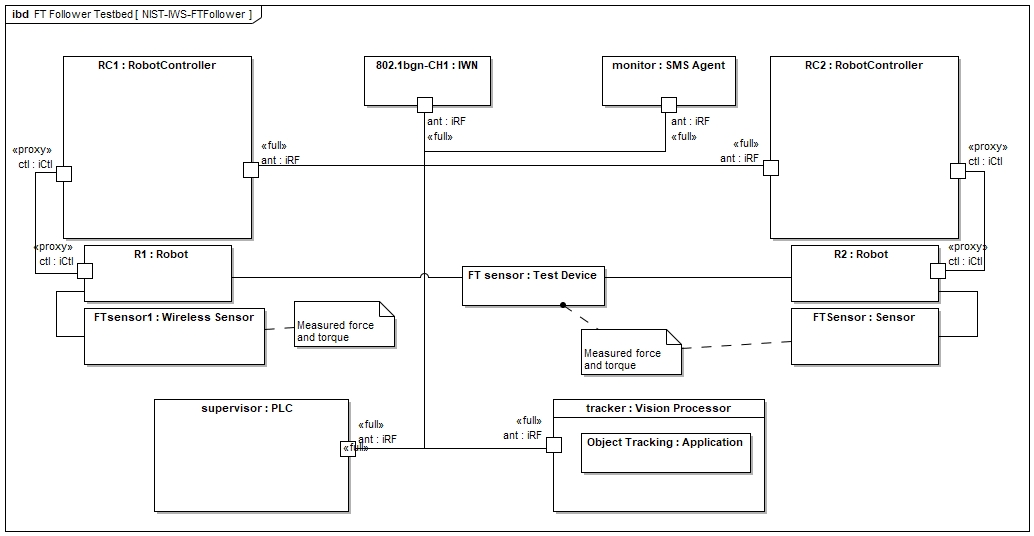
\includegraphics[width=0.85\textwidth]{chapter-conclusions/images/NIST-IWS-FTFollower}
	\caption{Internal block diagram of a workcell equipped with an robotic leader-follower lift application.}
	\label{fig:concl:lfscenario-full}
\end{figure}

\begin{figure}[!th]
	\centering
	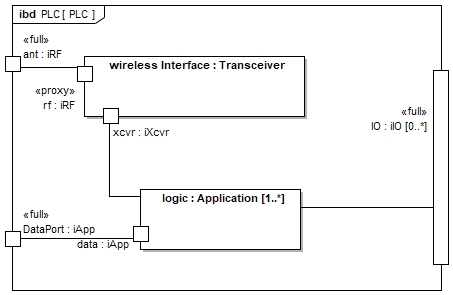
\includegraphics[width=0.85\textwidth]{chapter-conclusions/images/PLC}
	\caption{Internal block diagram of a PLC.}
	\label{fig:concl:plc-ibd}
\end{figure}

\begin{figure}[!th]
	\centering
	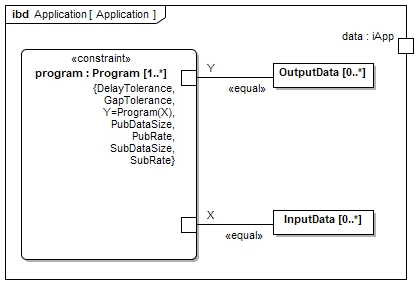
\includegraphics[width=0.85\textwidth]{chapter-conclusions/images/Application}
	\caption{Internal block diagram of an Application showing the parametrics constraints of its one or more programs.}
	\label{fig:concl:Application-ibd}
\end{figure}

\begin{figure}[!th]
	\centering
	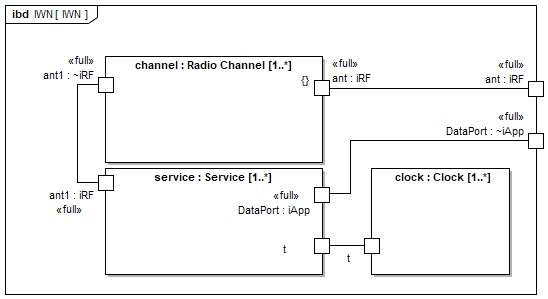
\includegraphics[width=0.85\textwidth]{chapter-conclusions/images/IWN}
	\caption{Internal block diagram of an Industrial Wireless Network (IWN) showing the parametric constraints of its one or more programs.}
	\label{fig:concl:iwn-ibd}
\end{figure}

\begin{figure}[!th]
	\centering
	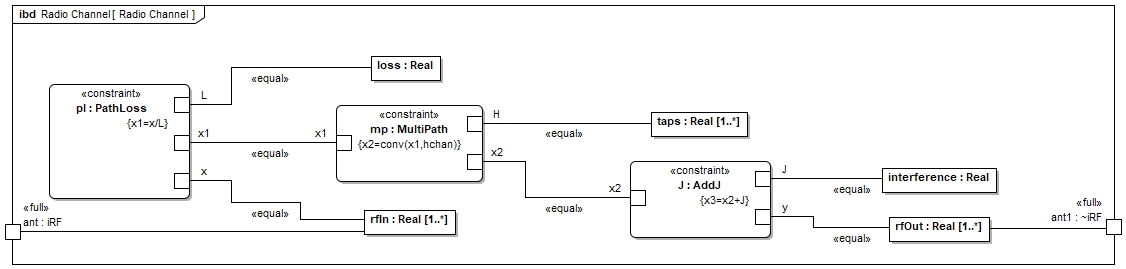
\includegraphics[width=0.85\textwidth]{chapter-conclusions/images/RadioChannel}
	\caption{Internal block diagram of an Radio Channel showing the parametric constraints of the radio medium.}
	\label{fig:concl:RadioChannel-ibd}
\end{figure}

\begin{figure}[!th]
	\centering
	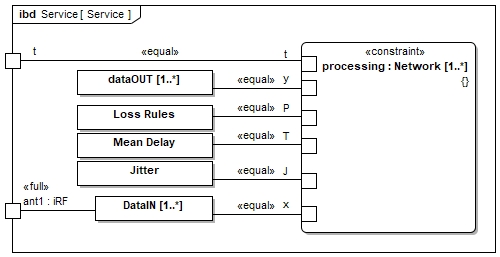
\includegraphics[width=0.85\textwidth]{chapter-conclusions/images/Service}
	\caption{Internal block diagram of an IWN Service showing the parametric constraints of the behavior of a network service as generic processing.}
	\label{fig:concl:Service-ibd}
\end{figure}

And as shown in Fig.~\ref{fig:concl:conceptual}, each controller block such as a Robot Controller or a PLC~(Fig.~\ref{fig:concl:plc-ibd}) inherits its structure and behavior from the Controller block.  As such, the PLC and the Robot Controller have an Application and an interface the to the wireless network.  Each application is linked to the wireless network through a Transceiver block (refer to \ref{fig:concl:plc-ibd}) which intuitively governs its own receiver performance as impacted by the radio channel.  The radio channel is an element of the IWN block shown in Fig.~\ref{fig:concl:iwn-ibd} which is connected directly to a set of IWN services as shown in Fig.~\ref{fig:concl:Service-ibd}. The service block of the IWN is modeled as a generic sets of contraints that could be implemented as code or mathemetical limitations.  

One can clearly see that the complete path of information flow within the model proposed traverses the radio medium, the industrial wireless network, the embedded transeivers, and each control application. Therefore, it is possible using this proposed model to represent the radio channel, model its performance impacts on the wireless network, and subsequently the impacts of the performance of the wireless network on the performance of the control applications themselves.  This is not an easy prospect and could be quite challenging for an engineer attempting to do so; however with the model presented, it is quite possible.  This represents an opportunity for refinement of the proposed model to be more intuitive and perhaps easier to use.  The contribution is made publically available through Internet download through the URL provided in~\cite{Candell2018SysML.DATA}.

\begin{figure}[!th]
	\centering
	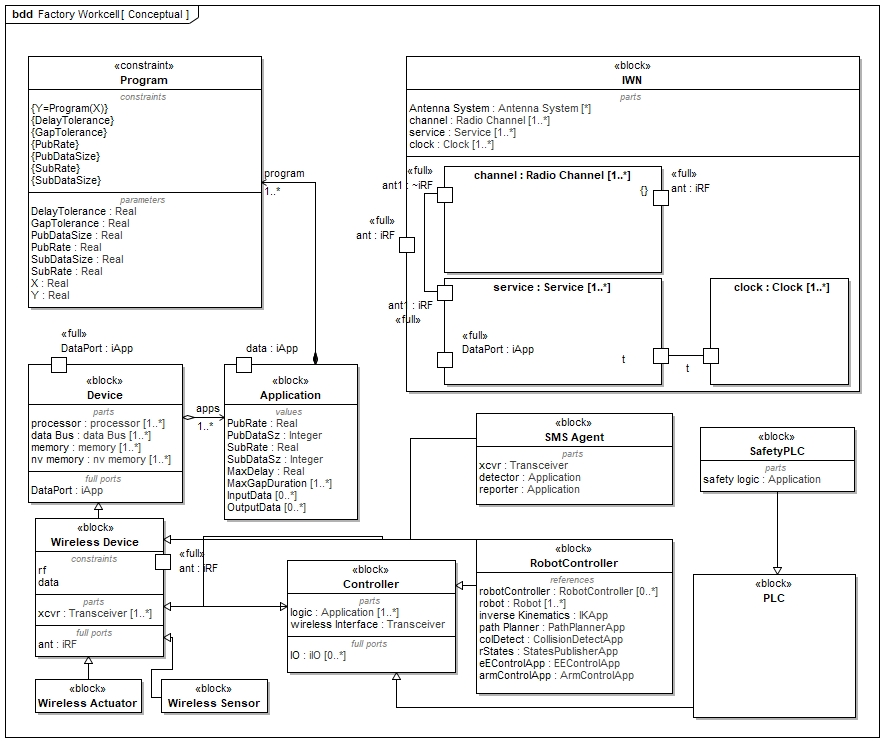
\includegraphics[width=0.85\textwidth]{chapter-conclusions/images/Conceptual}
	\caption{BBD of the conceptual relationships of model primitives}
	\label{fig:concl:conceptual}
\end{figure}

 that impact performance of the supporting network and subsequently the phys.

A model was developed using SysML. The developed model is constructed of the elements necessary to construct useful representations of factory work-cells in which wireless networks are used to transport information necessary for automated control system operation.  Reusable, derivable elements are developed and then extended to represent the constructs of the work-cell such as robot control, supervisory control, vision, safety, and spectrum monitoring.  An industrial wireless network is then developed and constraints of the radio channel and network services are formalized. Using the architectural model, information flows are explored and incorporated within. 

It is important to mention that this model includes an often overlooked component of any industrial wireless deployment which is the spectrum monitoring system and also considers the human-robot and robot-robot interactions in industrial environments. The current model includes various systems constraints including motion constraints, radio channel constraints, and networking constraints. The parametric constraints are provided as examples and can be replaced with executable computer code thereby making the model useful for simulation depending on the modeling tool selected. Furthermore, the applications within the robotic work-cell define many information flows requiring careful analysis to achieve reliability and latency necessary for the safety and control of the manufacturing process.

With increased dependency on wireless communications for more complex manufacturing systems, the projection of manufacturing requirements onto the wireless communication system becomes less obvious. Such analysis of this projection is essential for future research of manufacturing systems. As such, the architectural elements and information flows exposed by an abstract model
are a necessary first step. The model in its current state of development is comprehensive enough to support architectural and ontological analyses of the factory work-cell.  As such, information about the relationships between components of a work-cell and attributes related to the wireless network may be discovered. Therefore, the model serves as a foundation for future systems engineering analyses. Moreover, the model may be used as a tool for academic and industry exploration of wireless testbed development.  The model is made openly available through GitHub at~\cite{SysML.Candell2018}.

\subsection*{Graph Database Application}

recall what was presented

proof that wireless performance does not severely impact physical system performance
would be interesting through simulation using the sysml model how the wireless network performance impacts the performance of the physical system and compare that to the empiral results. 

\subsection*{Machine Learning Applications}



\section{Future Opportunities}
Move the future work sections here
\subsection*{Requirements Mapping}
\subsection*{Modeling using SysML}
\subsection*{Graph Database Application}
\subsection*{Machine Learning Applications}

%\chapter{Conclusions}
%
%\section{Future Work}
%Application of Machine Learning within the workcell control program
%
%how to extended the graph database and other data management approaches to the the factory and factory workcell rather than just for performance appraisal in the lab.
%
%Improvements to the schema, queries, and other database improvements to overcome the challenges encountered during research.  For example, rapidly expanding cartesian products within queries.  I note that the selected database has inherent problems with large scale queries wherein a query is constructed to for efficiency yet the database ignores the rules of the query and forms a cartesian product regardless.
%
%\section{Conclusions}

%\include{chapter-conclusions/chapter-conclusions}


%\chapter{Conclusions}
%paper on testbed construction; ground truth; data sources network and physical; data outputs; 
%paper on graph database approach for organization of data
%Discussion, Perspectives, restate findings
